\documentclass[border=4pt,12pt]{standalone}
% House style for redrawn exam diagrams (diagram-v4: 0.4pt lines, filled -latex arrows, fine dashes; stipple and hatching drawn as real dots/lines (no PDF/SVG patterns, so they render in every browser and at any scale); transparent background). Every figure \input's this.
\usepackage{amsmath,amssymb}
\usepackage{txfonts}
\usepackage{pdfrender,xcolor}
% \halo{text}: label on shading. The shading stops just around each letter's outline (a thin knock-out that follows the
% glyphs, like the papers' typesetting), never a box. Owner: "I don't want a box around the text".
\newcommand{\halo}[1]{\leavevmode\rlap{\pdfrender{TextRenderingMode=2,LineWidth=2.2pt,LineJoinStyle=1,StrokeColor=white,FillColor=white}#1}#1}
\usepackage{tikz,pgfplots}
\pgfplotsset{compat=1.18}
\usetikzlibrary{arrows.meta,calc,angles,quotes,patterns,patterns.meta,intersections,positioning,decorations.markings,shapes.geometric}
% Stipple and hatching are drawn as actual dots / lines clipped to the region (path picture), NOT as pattern fills:
% SVG <pattern> fills vanish or blur when browsers scale the image, so the owner could not see the shading.
% Each dot is a 0.72pt square (keeps SVGs small; reads as a dot at print size). Dots sit on one global staggered grid, so neighbouring regions line up.
\makeatletter
\newdimen\ex@x \newdimen\ex@y \newdimen\ex@xa \newdimen\ex@ya \newdimen\ex@xb \newdimen\ex@yb \newcount\ex@row
\def\exam@stipplecolor{black!75}\def\exam@dotr{0.42pt}\def\exam@dotgap{2.5}
\def\ex@rowdots{\ifdim\ex@x<\ex@xb \pgfpathrectangle{\pgfqpoint{\dimexpr\ex@x-0.36pt\relax}{\dimexpr\ex@y-0.36pt\relax}}{\pgfqpoint{0.72pt}{0.72pt}}\advance\ex@x by \exam@dotgap pt\relax\expandafter\ex@rowdots\fi}
\def\exam@stipple{%
  \pgftransformreset% dots are sized in real points even inside scaled pictures
  \pgfpointanchor{path picture bounding box}{south west}\ex@xa=\pgf@x \ex@ya=\pgf@y
  \pgfpointanchor{path picture bounding box}{north east}\ex@xb=\pgf@x \ex@yb=\pgf@y
  \pgfsetfillcolor{\exam@stipplecolor}\pgfmathsetmacro\ex@h{\exam@dotgap/2}%
  \pgfmathtruncatemacro\ex@r{floor(\ex@ya/\ex@h)-1}\ex@row=\ex@r\relax
  \ex@y=\ex@r\dimexpr\ex@h pt\relax
  \loop\ifdim\ex@y<\ex@yb
    \pgfmathtruncatemacro\ex@c{floor(\ex@xa/\exam@dotgap)-1}\ex@x=\ex@c\dimexpr\exam@dotgap pt\relax
    \ifodd\ex@row \advance\ex@x by \ex@h pt\fi
    \ex@rowdots
    \advance\ex@y by \ex@h pt \advance\ex@row by 1
    \ifnum\numexpr\ex@row-(\ex@row/4)*4\relax=0 \pgfusepath{fill}\fi% flush every 4 rows: bounded TeX memory, few clip copies in the SVG
  \repeat\pgfusepath{fill}}
\newdimen\ex@d
\def\exam@hatch#1{% #1 = 1 for /, -1 for \ ; lines 45 degrees, 3pt apart
  \pgftransformreset
  \pgfpointanchor{path picture bounding box}{south west}\ex@xa=\pgf@x \ex@ya=\pgf@y
  \pgfpointanchor{path picture bounding box}{north east}\ex@xb=\pgf@x \ex@yb=\pgf@y
  \ex@d=\dimexpr\ex@yb-\ex@ya\relax \ex@x=\dimexpr\ex@xa-\ex@d\relax
  \loop\ifdim\ex@x<\ex@xb
    \ifnum#1>0 \pgfpathmoveto{\pgfqpoint{\ex@x}{\ex@ya}}\pgfpathlineto{\pgfqpoint{\dimexpr\ex@x+\ex@d\relax}{\ex@yb}}%
    \else \pgfpathmoveto{\pgfqpoint{\ex@x}{\ex@yb}}\pgfpathlineto{\pgfqpoint{\dimexpr\ex@x+\ex@d\relax}{\ex@ya}}\fi
    \advance\ex@x by 4.24pt
  \repeat
  \pgfsetlinewidth{0.4pt}\pgfsetstrokecolor{black}\pgfusepath{stroke}}
\def\examstipple{\exam@stipple}\def\examhatch{\exam@hatch}\def\examsetstipplecolor#1{\def\exam@stipplecolor{#1}}\def\examsetdotgap#1{\def\exam@dotgap{#1}}
\makeatother
% (legacy pattern kept for old files)
% staggered stipple like the NESA papers' dotted shading
\pgfdeclarepatternformonly{exam stipple}{\pgfpointorigin}{\pgfqpoint{2.2pt}{2.2pt}}{\pgfqpoint{2.2pt}{2.2pt}}{%
  \pgfpathcircle{\pgfqpoint{0.55pt}{0.55pt}}{0.42pt}\pgfpathcircle{\pgfqpoint{1.65pt}{1.65pt}}{0.42pt}\pgfusepath{fill}}
\tikzset{
  every picture/.style={line width=0.6pt, >={Latex[length=2mm,width=1.3mm]}},
  curve/.style={line width=0.6pt},
  open arrow/.style={-{Latex[length=2mm,width=1.3mm]}},  % owner: filled -latex heads everywhere, no open chevrons
  aux/.style={dash pattern=on 2pt off 1.5pt, line width=0.6pt},
  shade/.code={\def\exA{#1}\def\exB{none}\ifx\exA\exB\else\pgfkeysalso{fill=black!18}\fi},
  shade/.default=on,
  shade dots/.style={fill=none, path picture={\examstipple}},
  stipple color/.code={\examsetstipplecolor{#1}},
  stipple gap/.code={\examsetdotgap{#1}},
  shade dense dots/.style={fill=none, stipple gap=1.6, path picture={\examstipple}},
  shade hatch/.style={fill=none, path picture={\examhatch{1}}},
  shade hatch reverse/.style={fill=none, path picture={\examhatch{-1}}},
  shade solid/.style={fill=black},
  pt/.style={circle, fill, inner sep=1.1pt},
  open pt/.style={circle, draw, fill=white, inner sep=1.1pt},
}
\pgfplotsset{
  exam axes/.style={axis lines=middle, axis line style={->}, xlabel={$x$}, ylabel={$y$},
    xlabel style={anchor=west}, ylabel style={anchor=south}, tick label style={font=\small},
    every axis plot/.append style={line width=0.6pt, black}, samples=200, clip=false,
    enlargelimits=false, axis on top},
}

\begin{document}
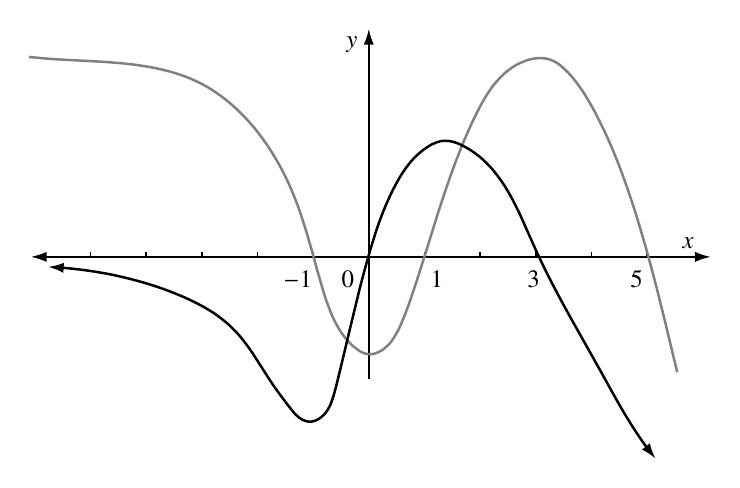
\begin{tikzpicture}[x=0.0127cm,y=-0.0127cm]
  \draw[<->] (35,270)--(715,270);
  \draw[->] (373,392)--(373,42);
  \foreach \k in {-5,...,-1,1,2,...,5}\draw (373+55.7*\k,270)--(373+55.7*\k,265);
  \draw[black!50,line width=0.9pt] plot[smooth] coordinates {(33,70) (56.71,72.1) (82.05,73.48) (107.6,74.88) (131.7,76.91) (154.1,80.1) (175.2,84.92) (194.2,91.48) (211.6,100.1) (228,111.2) (243.2,124.4) (257.6,139.9) (270.6,157.1) (282.2,175.7) (292.3,195.4) (300.9,216) (308.5,238.2) (315.6,262.2) (322.5,287.1) (329.4,310.3) (336.7,329.7) (345.3,345.4) (355,357.2) (365,364.9) (371.9,367.3) (378.3,366.9) (386.5,363.2) (394.5,355.9) (402.4,343.4) (410.4,324.6) (418.5,301.4) (426.3,277.2) (434.2,252) (441.9,227.2) (449.9,203) (458.1,179.7) (467,156.9) (476.6,135.1) (486.8,115) (497.3,98.87) (508.6,86.57) (520.6,77.95) (533.5,72.62) (545.1,71.08) (554.6,72.72) (563.8,77.8) (575,88.42) (586.9,104.1) (597.8,122.5) (608.4,143.5) (618,165.2) (626.9,188) (635.1,211.4) (642.7,235.3) (649.8,259.5) (656.6,284.2) (663,309) (669.2,334.1) (675.4,359.9) (681.6,385.4)};
  \draw[<->,line width=0.9pt] plot[smooth] coordinates {(52,280) (72.44,281.4) (92.52,283.8) (112.5,287.1) (132.2,291.5) (151.5,296.8) (170.5,303.2) (188.6,310.5) (205.2,318.6) (220,327.6) (233.1,338) (244.2,349.5) (254.8,363.5) (266.1,380.9) (277.3,398.2) (289.5,414.9) (299.6,427.5) (306.2,432.7) (311.9,434.7) (316.9,434.6) (322.7,432.3) (328.7,427.3) (333.8,419.6) (338.3,407) (343.6,386.1) (348.8,364.5) (354,342.6) (359.3,320.7) (364.5,299.5) (370.1,278.5) (376,258) (382.3,238.3) (389.4,219.8) (397.3,202.6) (406,187.1) (415.3,174.4) (425.4,164.6) (436.1,157.4) (444.6,154.3) (452.2,153.9) (461.7,156.3) (473.6,162.4) (485.7,171.3) (496.6,182.3) (506.7,195.6) (516,211.1) (524.7,228.6) (533.5,248.4) (542.4,268.1) (551.6,287.1) (561.6,306.4) (572,325.6) (582.8,344.9) (593.8,364.5) (604.7,383.9) (615.6,403.6) (626.3,422.5) (637,440) (648.3,456.8) (660,472)};
  \node[font=\small] at (356,58) {$y$};
  \node[font=\small] at (692,256) {$x$};
  \node[font=\small] at (302,292) {$-1$};
  \node[font=\small] at (352,292) {$0$};
  \node[font=\small] at (441,292) {$1$};
  \node[font=\small] at (538,292) {$3$};
  \node[font=\small] at (641,292) {$5$};
\end{tikzpicture}
\end{document}
